
\section{Agent Controllers\label{sec:SystemFeaturesAgentControllers}}

The purpose of the agent controllers is to be able to control agents
in the engine from outside. This section will cover our setup of an
agent controller. 

To get an overview of the classes used for the \texttt{AgentController},
look at fig. \ref{fig:AgentControllerDomainModel}.

\begin{figure}
\begin{centering}
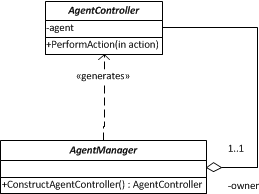
\includegraphics[width=0.7\textwidth]{AgentControllerDomainUML}
\par\end{centering}

\caption{Domain model for Agent Controller\label{fig:AgentControllerDomainModel}}
\end{figure}



\subsection{Concept}

The engine is designed to support the ability to be adapted for all
APL types, this means that the engine itself does not support all
APLs but instead provides a framework for quickly designing interfaces
between the engine and any APL. There are two classes that one must
use in order to properly design the interface:
\begin{description}
\item [{The~\texttt{AgentManager}}] has the duty of speaking directly
with the agent language it attempts to interface with. Its job is
to spawn an \texttt{AgentController} for each agent the AP wishes
to take control of. The \texttt{AgentManager} is in that sense much
akin to an Abstract Factory (see sec. \ref{sec:TheoryFactoryDesignPattern})
, which -- according to the design pattern -- is an abstract class
with a method generating a certain type of object, without restricting
exactly which object is generated, as long as it is of the specified
type. The idea is that if you have a \texttt{GoalAgentManager} then
the controller it constructs would be \texttt{GoalAgentController}.
The methods required by both the \texttt{AgentController} and the
\texttt{AgentManager} are abstract. Thus, we ensure at compile time
that the engine framework is properly used\texttt{\emph{.}}
\item [{The~\texttt{AgentController}}] is the link between a single agent
and the AP. Its job is to take all commands sent to it by the connected
AP, transform them into actions understood by the engine, and apply
them to the agent that it controls.
\end{description}
To simplify the \texttt{AgentController} design, it provides the method
\texttt{PerformAction}, which makes it easy to execute actions on
the agent it controls. When the \texttt{PerformAction} is called,
the \texttt{AgentController} queues the action given through the method
and puts the \texttt{AgentController}\textquoteright{}s thread to
sleep. Once the action has been executed by the engine, the \texttt{AgentController}
is woken up and returns from the \texttt{performAction} method. All
percepts received by the \texttt{AgentController} during this time
is stored on the \texttt{AgentController} and can be easily accessed
by the actual implemenation of the \texttt{AgentController}.

\begin{figure}
\begin{centering}
\includegraphics[width=0.95\textwidth]{AgentManagerAndAgentControllSequenceDiagram}
\par\end{centering}

\caption{This sequence diagram shows the process of an AP taking control of
agent through the \texttt{AgentManager}, and commanding it through
the \texttt{AgentController\label{fig:APConnectingToAndControllingAC}}}
\end{figure}


The process of an AP taking control of an agent is illustrated in
fig. \ref{fig:APConnectingToAndControllingAC}. The AP calls the \texttt{AgentManager}
to locate the agent it wishes to assume control of. The agent is located
through a string (its name) which is unique to it and ensures that
only one agent is taken. When the \texttt{AgentManager} finds the
correct agent, it will immediately generate a new \texttt{AgentController}.
The AP will not gain access to the agent but instead it will gain
access to the \texttt{AgentController}. Now that the AP possesses
the \texttt{AgentController}, it will have the ability to send the
\texttt{AgentController} commands. These commands might not be understood
by the engine if the APL is foreign enough to the engine\textquoteright{}s
own language and as such it is the duty of the \texttt{AgentController}
to convert these commands into actual actions which the engine can
understand.


\subsection{How to use agent controllers}

To use the built-in controller features of the engine, the designer
must provide his own implementations of \texttt{AgentController} and\texttt{
AgentManager}. The designer must do this for every different APL he
wishes to use in the engine.

The classes \texttt{AgentManger} and \texttt{AgentController} both
provides functionality as part of their own classes but also requires
some methods that must be implemented for the classes to function.

For the \texttt{AgentManager }the designer must provide a method that
produces \texttt{AgentControllers} of their implemention, along with
locating an agent though the \texttt{AgentManager} does provide some
assistance in that regard, in the form of a agent locating method
defined as: \texttt{TakeControlOf}, which takes the name of an agent
as a string, and returns the corresponding \texttt{Agent}. Furthermore,
it should be noted that the \texttt{AgentManager} is also automatically
designed to create threads for the \texttt{AgentControllers} it constructs.

For the \texttt{AgentController}, the designer must provide all logic
defining how a controller handles a given agent, this means getting
the percepts from the agent, analyzing the percepts and deciding an
action (Could be outsourced to another APL such as GOAL) and then
queue said action to the agent. The AgentController has the method
\texttt{PerformAction}. This method can be very useful as it queues
an action automatically to its agent, then blocks the thread until
the action has been performed. Furthermore, this action will also
trigger a C\# event called \texttt{PerceptsRecieved} in the case that
the agent controller actually recieve any percepts during the action.
For instance, this event could be used for where the \texttt{AgentController},
decides the next action for the agent to perform, as done in the Vacuum
World Example in appendix \ref{chap:VacuumWorldAppendix}.


\subsection*{Summary}

The agent controller is designed to be very lightweight, since we
do not want to impose any restrictions that might limit an APL which
we know nothing about. As such, the \texttt{AgentController} is more
akin to a convention or a design pattern for how interfacing with
agents should occur. It provides the skeleton of how a link might
be designed but does not impose any restriction on how the link should
be set up.
